\subsection{Quantum Chromodynamics (QCD)}

% OVERVIEW
%
%   * a theory of the strong interaction (color force)
%   * It is the study of the SU(3) Yang�Mills theory of color-charged fermions (the quarks)  
%   * Described by the SU(3) group
%   * QCD is a gauge theory of the SU(3) gauge group obtained by taking the color charge to define a local symmetry. 


QCD is a physical theory that describes the interactions between particles with the property of colour via strong interactions. It is a gauge theory with a symmetry group of SU(3) (the group of unitary matrices with a determinant of one) and describes the interactions between quark and gluon fields. 

The strong force is responsible for the binding force which holds nucleons together to form the nucleus of an atom. This is due to the deeper fundamental interaction between the components of nucleons - quarks and gluons - collectively called partons. The gluons are the gauge bosons of the theory i.e. mediators of the strong force. It is a short range force having a significant effect only on scale of $\sim1$ fm (about the size of the charge radius of a proton) due to the nature of its coupling. The Lagrangian of QCD is,

\begin{equation}
	\mathcal{L} = \bar\psi_i i((\gamma^\mu D_\mu)_{ij} - m \delta_{ij})\psi_j - \frac{1}{4}G^a_{\mu\nu}G^{\mu\nu}_a
	\label{equation: qcd lagrangian}
\end{equation}

where $\bar\psi_i$ is the quark field and $G^a_{\mu\nu}$ is the gluon field strength tensor given by,

\begin{equation}
	G^a_{\mu\nu} = \partial_\mu A^a_\nu - \partial_\nu A^a_\mu + gf^{abc} A_\mu^b A_\nu^c
\end{equation}

where $A^a_\nu$ are the gluon fields and $f^{abc}$ are the fine structure constants of the SU(3) group.

%BOUND STATES
Quarks have been observed in two-quark bound states (mesons) and three-quark bound states (baryons); the six flavours of quarks give rise to many possible quark combinations, these combinations are commonly grouped into octets by the eightfold way, figure \ref{fig: eightfold way}.


%\subsection*{Parton Bound States}
%The three colours form a quark triplet, 

%\begin{equation}
%	c = \[
%	\left(
%	\begin{array}{c}
%		\psi_1 \\
%		\psi_2 \\
%		\psi_3   
%	\end{array}
%	\right)
%	\]
%\end{equation}

\begin{figure}[h]
	\begin{subfigure}[h]{0.49\textwidth}
		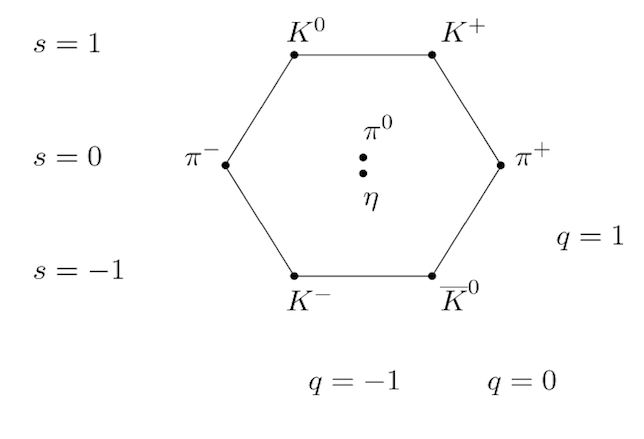
\includegraphics[width=\textwidth]{./Chapters/theory/standard_model/images/meson_octet.png}
		\caption{The meson octet (two quark bound states)}
		\label{fig: meson octet}
	\end{subfigure}
	\begin{subfigure}[h]{0.49\textwidth}
		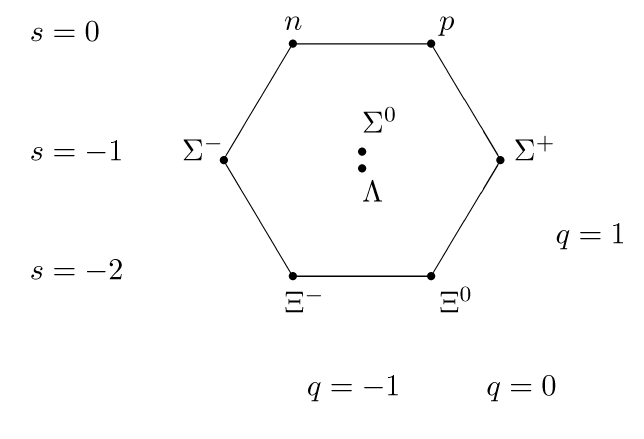
\includegraphics[width=\textwidth]{./Chapters/theory/standard_model/images/baryon_octet.png}
		\caption{Baryon octet (three quark bound states)}
		\label{fig: baryon decuplet}
	\end{subfigure}
	\caption{Eightfold method of organising quark bound states. Bound states on the same horizontal share the same strangeness and those on the same diagonals running top left to bottom right share the same charge}
	\label{fig: eightfold way}
\end{figure}

% COLOUR
The property of colour in QCD is analogous in many ways to the role of electric charge in QED. However instead of there being one type of charge in QCD there are three types, labelled red, green, blue and their corresponding anti-colours anti-red, anti-green and anti-blue. The names of the charge types are motivated by the behaviour of coloured light such that a bound state of a red, blue and green quarks gives a net colour charge of white or colourless; a combination of colour and anti-colour is also colourless.

% PARTONS
Each quark possesses one of the three types of colour charge; it can be either red, green or blue (similarly so for anti-quarks and the anti-colour charges). Gluons on the other hand possess a combination of colour and anti-colour charge (though these charges are not necessarily of the same colour). Since gluons are charged, QCD features some additional richness not seen in its QED counterpart. Gluons can couple with one other unlike photons which cannot, see figure \ref{fig: qcd field couplings}.

\begin{figure}[h]
	\centering
	\begin{subfigure}[h]{0.32\textwidth}
		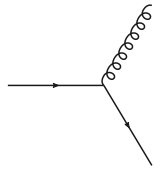
\includegraphics[width=0.8\textwidth]{./Chapters/theory/standard_model/images/quark_gluon.png}
		\caption{Quark-gluon vertex}
		\label{fig: quark-gluon vertex}
	\end{subfigure}
	\begin{subfigure}[h]{0.32\textwidth}
		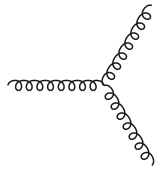
\includegraphics[width=0.8\textwidth]{./Chapters/theory/standard_model/images/gluon3.png}
		\caption{Three-gluon vertex}
		\label{fig: three-gluon vertex}
	\end{subfigure}
	\begin{subfigure}[h]{0.32\textwidth}
		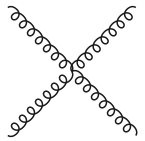
\includegraphics[width=0.8\textwidth]{./Chapters/theory/standard_model/images/gluon4.png}
		\caption{Four-gluon vertex}
		\label{fig: four-gluon vertex}
	\end{subfigure}
	\caption{QCD field couplings}
	\label{fig: qcd field couplings}
\end{figure}

\subsection*{Asymptotic freedom}
The coupling constant $\alpha_s$ of QCD describes the strength of the strong interaction. The $\beta$ function for the strong coupling constant is given by,

\begin{equation}
	\beta(\alpha_s) = - \left(11 - \frac{2n_f}{3}\right)\frac{\alpha_s^2}{2\pi}
\end{equation}
where,
\begin{equation}
	\alpha_s = \frac{g^2}{4\pi}
\end{equation}

and $n_f$ is the number of quark flavours in the theory. Since there are six quark flavours in the standard model the values of the $\beta$ function are negative i.e. the coupling constant of the strong force decreases with an increase in the energy transfer (or equivalently a decrease in the distance) of the process. The running coupling constant as a function of the energy transfer is given by,

\begin{equation}
	\alpha_s(|q^2|) = \frac{4\pi}{(11 - \frac{2n_f}{3})\mathrm{ln}(|q^2|/\Lambda^2)} \,\,\,\,\,\, (|q^2| >> \Lambda^2)
\end{equation}

where $|q^2|$ is the energy transfer of the process and $\Lambda$ is the QCD scale defined as the energy transfer at which the strong coupling constant $\alpha_s \sim 1$ and perturbative calculations with expansions of the coupling constant diverge.

This behaviour of the strong force coupling constant to become weaker at short range interactions is known as asymptotic freedom. Quarks and gluons which interact over short distances - such as at high energy collider experiments - interact very weakly and act as quasi-free particles. Since the coupling constant is small in this regime perturbative methods can also be used calculate properties of the theory.

\subsection*{Colour Confinement}
Colour confinement is an observed phenomenon in which partons are only observed in bound colour singlets states, i.e. no individual free quarks or gluons have been observed. As quarks are separated the coupling constant increases such that the energy needed to separate them increases indefinitely. At some energy threshold the system of separating quarks will have enough enough energy to spontaneously form quark anti-quark pairs - forming a bound state with the initial quarks. This process - called hadronisation - may occur multiple times resulting in a shower of particles called a jet. Since the strong coupling constant is inherently large in these processes perturbative methods are incompatible with describing this behaviour, instead our best understanding is achieved by phenomenological models (see section \ref{section: hadronisation}). 

%\input{./Chapters/theory/standard_model/qcd_factorisation_theorem}

% and lattice QCD which is based on the principle of quantising space and time into a lattice. 

%Colour confinement is deeply tied into understanding particle production in particle collision experiments. In the case of a scattering experiment of a composite object without components such as photon-electron scattering in an atom, the energy transfer may result in the electron being freed from the atom overcoming the electromagnetic attractive forces (the photoelectric effect). However in the case of coloured objects such as quarks this does not occur. In the theory of QCD quark-quark interactions from proton-proton collisions with large enough energies to separate the initial quarks in a proton by a threshold distance resulting in the spontaneous production of quark-antiquark pairs, each quark binding with either of the other quarks in the proton or with the separated quark such that only composite objects are present in the final state of the interaction.

%The phenomena of colour confinement and asymptotic freedom pose many challenges for physicists due primarily to the behaviour of the strong coupling constant. Unlike the coupling constants for the electromagnetic and weak interactions increases with distance between correspondingly charged particles. Perturbative calculations expanded about the strength of the coupling constant diverge meaning the calculations become invalid.

%When quarks in bound states such as mesons and baryons are separated from each other, the increasing strength of the strong interaction between them may result in the spontaneous creation of quark-antiquark pairs, these are generally referred to as showers or jets of hadrons. Since the strong coupling constant is large in these processes it is not possible to calculate the probability of these processes from the fundamental Lagrangians of the Standard Model. Instead separate hadronisation models such as the Lund String model discussed in section \ref{section: hadronisation} are used instead. Ideally jet behaviour would be described by the Lagrangians of the Standard Model, however a complete understanding of this behaviour still has its challenges - though much progress has been made by hadronisation models.


% SU(3)

% LAGRANGIAN 
%These interactions correspond to the three and four gluon vertex diagrams seen in the Feynman diagram representation and by the corresponding Lagrangian terms (see equation \ref{equation: qcd lagrangian} and figure \ref{fig: qcd field couplings}).

